\chapter{\textit{Framework} de Avaliação da Qualidade do Código}

Este capítulo apresenta, inicialmente, o detalhamento das atividades do \textit{framework}. Por fim, apresenta-se os \textit{checklists} de implementação de testes unitários e inspeção de código obtidos a partir do referencial teórico.

\section{Detalhamento do \textit{Framework}}

Com base em todos os conceitos assimilados a partir da realização da revisão sistemática de literatura e também, da pesquisa bibliográfica, foi possível conceber um grupo de atividades que em sua totalidade compõem o \textit{framework} de avaliação de código.

Iniciando a descrição das atividades pelo macroprocesso, tem-se, conforme ilustrado na figura 3:

\begin{itemize}
	\item \textbf{Elicitar as proposições de valor:} Caracteriza-se como uma reunião entre todos os envolvidos no projeto (área de negócio e área técnica) para alinhamento da missão do projeto. Nesta reunião, a área de negócio irá descrever quais seriam as funcionalidades mais críticas e, portanto, que mais agregam valor em seu contexto, para o \textit{software} a ser construído, de forma que a equipe técnica possa efetuar um planejamento embasado neste aspecto.

	\item \textbf{Estabelecer os objetivos de teste e metas gerais de qualidade de código:} Nesta atividade, a equipe técnica irá conceber uma estratégia para testar e assegurar a qualidade do código do \textit{software} levando em consideração os módulos priorizados a partir da elicitação das proposições de valor.

	\item \textbf{Planejar sprints de implementação e execução dos testes e inspeções de código:} Nesta atividade, o gestor do projeto, juntamente com os representantes dos demais grupos técnicos existentes no processo de desenvolvimento irão planejar as sprints, definindo início e término das mesmas, bem como os módulos do código que serão testados e inspecionados de acordo com uma priorização obtida a partir das proposições de valor.

	\item \textbf{Verificar o planejamento da sprint a ser iniciada:} Nesta atividade, a equipe do projeto irá verificar as funcionalidades a serem desenvolvidas e o que deverá ser plenamente testado e inspecionado. Assim, fará a alocação apropriada dos recursos (humanos e financeiros) para atendimento dos objetivos da sprint.

	\item \textbf{Executar Sprint:} Subprocesso que compreende as atividades corriqueiras de uma sprint segundo o Scrum, contudo, acrescentando as atividades agregadas pelo \textit{framework}.

	\item \textbf{Revisar resultados da sprint:} Nesta atividade, a equipe técnica irá verificar se todos os objetivos estabelecidos para a sprint foram alcançados, ou seja, se de fato o que foi planejado foi executado. Caso seja necessário efetuar otimizações nos planejamentos, devido também à mudança de alguma proposição de valor, a primeira atividade deverá ser executada novamente. É válido ressaltar que a interação com o cliente deve ser intensa para promover a agregação de valor em um grau satisfatório. Adicionalmente, caso algum item fique pendente, este entrará imediatamente como algo a ser concluído na sprint subsequente.

	\item \textbf{Efetuar revisão geral do projeto:} Nesta atividade, haverá uma reunião entre as áreas de negócio e técnica e todas as proposições de valor serão apresentadas de forma breve, explicitando o planejamento e a execução. Caso alguma proposição fique pendente, será avaliada a possibilidade de prorrogação de prazo para término do projeto.
\end{itemize}

A figura a seguir ilustra o macroprocesso do \textit{framework} proposto.

\begin{figure}[h]
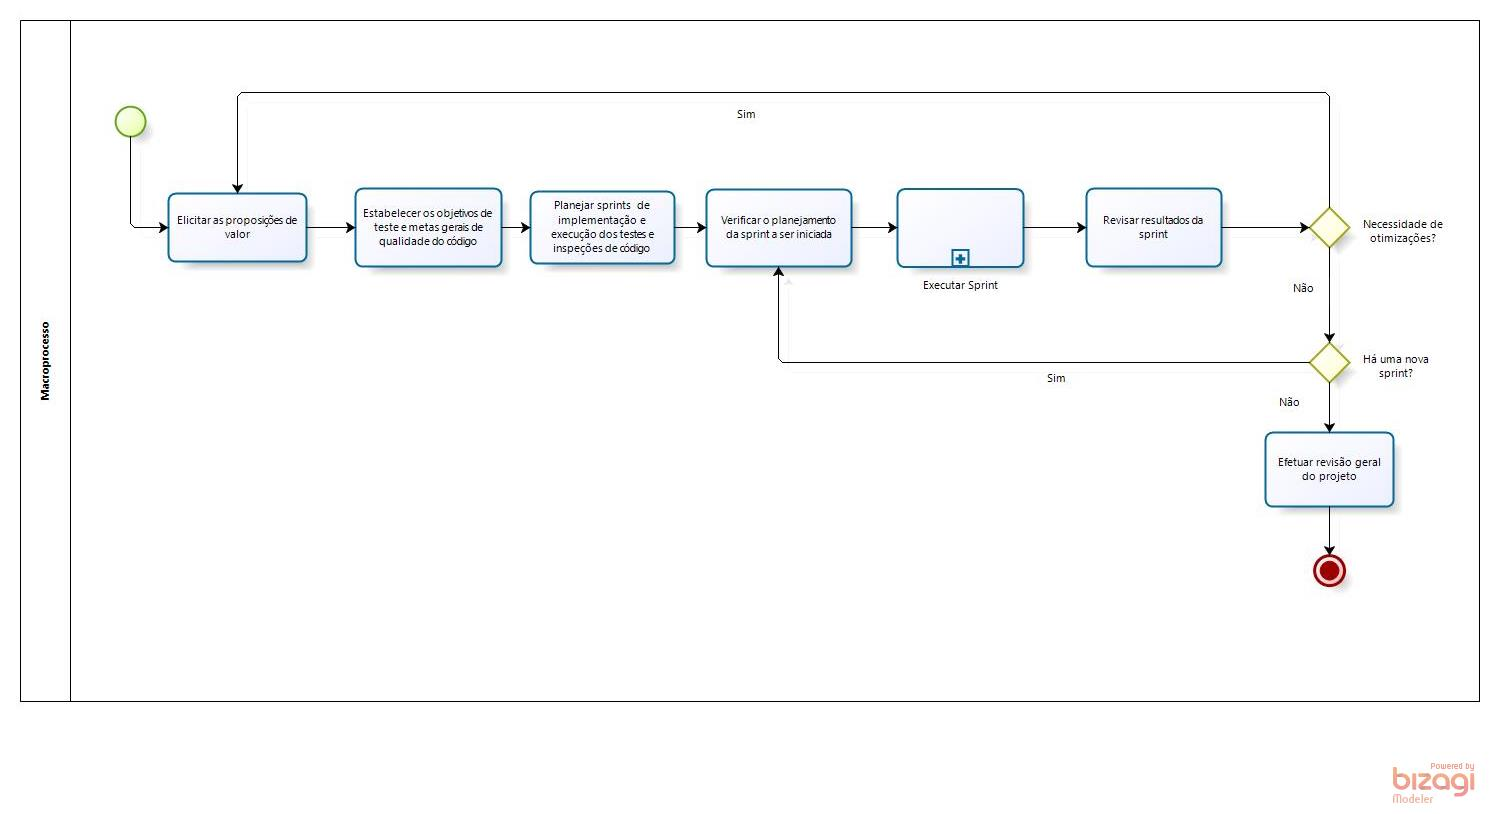
\includegraphics[width=\textwidth]{figuras/macroprocesso.jpg}
\caption{Macroprocesso - \textit{Framework de Avaliação de Código}}
\end{figure}

A partir da descrição das atividades, é possível perceber o quão importante é fazer um bom planejamento e priorização. Caso haja mudanças no escopo e também nos prazos, a princípio, as funcionalidades que mais agregam valor já terão sido cobertas pelos instrumentos de garantia de qualidade.

Quanto à descrição das atividades constituintes do subprocesso Executar Sprint, tem-se, conforme ilustrado pela Figura 4:

\begin{figure}[h]
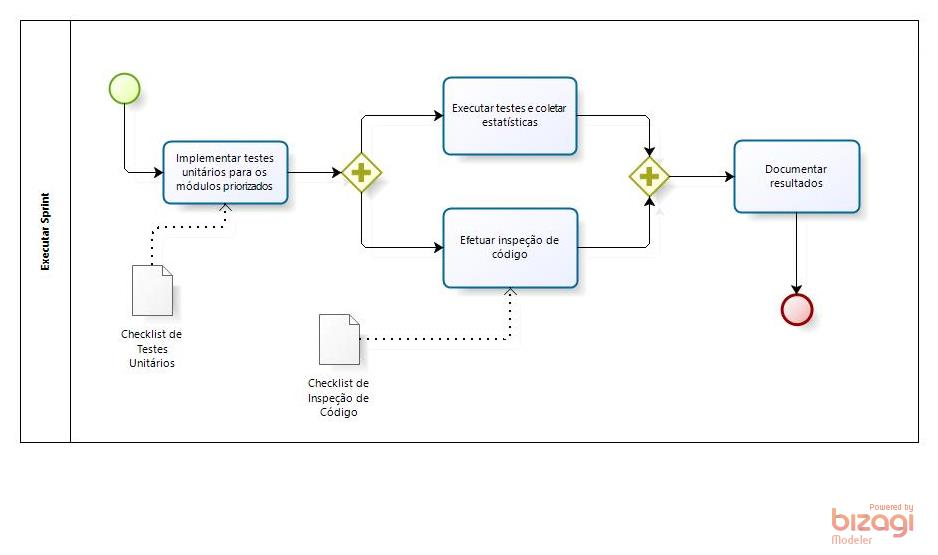
\includegraphics[width=\textwidth]{figuras/executarsprint.jpg}
\caption{Subprocesso - \textit{Executar Sprint}}
\end{figure}

\begin{itemize}
	\item \textbf{Implementar testes unitários para os módulos priorizados:} Esta atividade possui como entrada um \textit{checklist} de testes unitários, construído a partir da constatação de práticas utilizadas na indústria de desenvolvimento e que tem sido eficiente neste sentido. Assim, para a implementação dos testes unitários, espera-se o completo atendimento dos itens constantes neste \textit{checklist}.

	\item \textbf{Executar testes e coletar estatísticas:} Nesta atividade, a suíte de testes unitários será executada e aspectos pertinentes à execução desta serão coletados, de forma a verificar performance, número de defeitos detectados etc.

	\item \textbf{Efetuar inspeção de código:} Nesta atividade, deverá ser feita uma inspeção do código tanto dos módulos sob teste, como também do código dos próprios métodos de teste unitário, de forma a verificar a completude e atendimento aos itens constantes no \textit{checklist} de inspeção de código.

	\item \textbf{Documentar resultados:} Além da anotação das estatísticas coletadas durante a execução dos testes, será documentado o resultado da inspeção, explicitando para cada módulo avaliado o grau de qualidade. Em caso de detecção de erros e defeitos severos, o módulo não será aprovado, ou seja, considerado finalizado e assim, deverá ser feito o aperfeiçoamento do mesmo na sprint subsequente.
\end{itemize}

\section{\textit{Checklist} para Implementação de Testes Unitários}

O \textit{checklist} de implementação de testes unitários é composto dos seguintes itens, conforme a seção 2.3:

\begin{enumerate}
	\item Foram criados métodos de teste pequenos (máximo de 8 linhas de código)?
	\item Foram criadas convenções de nomenclatura para o código de teste (as classes, bem como os métodos de testes possuem nome condizente com o módulo que está sendo testado)?
	\item A suíte de testes é executada com êxito independentemente da ordem dos métodos de teste em execução?
	\item Os testes são auto verificáveis (já são utilizados mecanismos como assertivas e \textit{expected} de forma que a própria ferramenta de teste seja capaz de dizer se o teste passou ou não)?
	\item O código de teste segue uma estruturação hierárquica, sendo a mesma observada nas classes que constituem os componentes do \textit{software}?
	\item As funções mais internas aos métodos públicos das classes sob teste estão sendo devidamente testados pela suíte?
	\item Os \textit{stubs} são simples, pequenos e independentes de outros \textit{stubs} que simulam comportamentos de outros módulos?
	\item Foi utilizada ferramenta de análise de cobertura de código para verificar as linhas de código de fato exercitadas pela suíte de testes?
	\item Os métodos de teste elaborados foram capazes de exercitar todas as linhas e caminhos dos métodos da unidade sob teste?
	\item Foi analisada a \textit{performance} da suíte de testes quando esta foi executada, de forma a verificar consumo de memória e processamento?
\end{enumerate}

\section{\textit{Checklist} para Inspeção de Código}

O \textit{checklist} para inspeção de código é composto dos seguintes itens, conforme seção 2.2:

\begin{enumerate}
	\item Foi verificado o retorno de cada método?
	\item Foi verificado como são feitos os tratamentos de interrupções, bem como gerenciamento de regiões críticas (algumas aplicações exigem sincronização entre processos, visto que utilizam recursos compartilhados)?
	\item Foi verificado o comportamento de todos os trechos de código que são portadores de estruturas de repetição (\textit{for}, \textit{while} etc.)?
	\item Foi verificado como estão sendo tratadas as operações de entrada e saída de dados nos métodos das classes?
	\item Foi verificado o fluxo do programa, analisando as estruturas de controle(\textit{if}, \textit{else} etc.)?
	\item Foram verificados todos os trechos de código inutilizados?
	\item As atribuições de valores às constantes e às variáveis foram verificados?
	\item Os comentários do código foram verificados, assim como a legibilidade do mesmo (tal como nome de variáveis, métodos etc.)?
	\item Foram verificados os \textit{imports} e qualquer outro tipo de inclusão de código de outras bibliotecas?
\end{enumerate}